\section{Segregation of duties}

Questo concetto è molto importante.

La \textit{compliance} è più importante di \textit{security} perché bisogna 
essere conformi a degli standard.

È importante, come già detto in diversi punti degli appunti, separare i vari 
poteri delle persone, in maniera tale da assicurarsi che non avvengano ``abusi 
di potere''.

Network administrator concede i diritti, ma qualcuno deve autorizzare che il 
ruolo $x$ abbia i diritti. Il network administrator implementa la concessione. 
\todo{Sistema sta frase}


È importante anche che gli \textit{assets} vengano controllati. Solitamente gli 
\textit{assets} sono fisici, ma nel settore IT possono essere immateriali (come 
un file contente un disegno di un progetto per una architettura di rete). Quindi 
è importante documentare le responsabilità. Si è responsabili quando occorrono 
due condizioni:
\begin{itemize}
\item Quando si è nominati ufficialmente, tramite una delega formale
\item Si hanno i poteri per implementare correttamente quanto richiesto
\end{itemize}

\subsection{Personale}

Dal punto di vista della sicurezza il personale è sempre l'anello debole della 
sicurezza. I \textit{background check} dipende sempre in base alla mansione che 
dev'essere coperta. Questi controlli sono abbastanza sensibili, e di solito 
avvengono anche per ruoli come amministratore delegato.
Se viene maneggiato denaro o \textit{assets} sicuramente è necessario eseguire 
un \textit{background check} per assicurarsi la \textbf{professionalità} e 
l'\textbf{affidabilità} della persona. Anche essere coinvolti in una stupida 
rissa potrebbe compromettere l'affidabilità di una persona. I propri 
\textit{social network} quindi dovrebbero essere sempre controllati in maniera 
tale da non contenere contenuto non appropriato.

Il \textit{monitoring} delle email è un problema dappertutto tranne negli USA, 
perché lì le email non sono protette. L'azienda fa lo scanner dei PC dei 
dipendenti. In Italia, dopo un caso eclatante, la giurisprudenza permette di 
leggere le email di lavoro.

\subsubsection{Assunzione degli impiegati}

Bisogna fare attenzione quando si eseguono assunzioni del personale. È 
importante anche controllare che chi venga assunto non esegui manomissioni dei 
documenti ufficiali\footnote{La falsificazione di documenti nella pubblica 
amministrazione comporta una reclusione dai 2 ai 5 anni.}.

Il \textbf{mansionario} specifica cosa un impiegato deve fare.

\textit{Confidentiality agreement}: contratto in cui il lavoratore dichiara di 
non divulgare quello per cui lavora l'azienda e indica anche un limite di tempo 
per cui l'impiegato non può svolgere un lavoro nello stesso campo.


\subsubsection{Orientamento dei nuovi impiegati}


Quando un nuovo impiegato firma un documento:
\begin{itemize}
\item ha letto e accettato le policy di sicurezza
\item promette di non divulgare ID e password per il login
\item creare password di qualità
\item bloccare il terminale quando non è presente
\item riportare violazioni della sicurezza sospette
\item mantenere una buona sicurezza fisica
\end{itemize}

\subsubsection{Employee termination}

Quando si arriva al termine del periodo lavorativo si deve ritornare 
l'equipaggiamento aziendale e revocare l'accesso all'individuo. Badge e 
cartellini devono essere riconsegnati, e le autorizzazioni che l'individuo aveva 
all'interno dell'azienda devono essere revocate.

\subsection{Accordi tra terze parti}

Definiscono le \textit{policy} di sicurezza relative alle informazioni e le 
procedure per implementare le \textit{policy}; forniscono controlli per 
proteggersi contro software malevolo. Pubblicano restrizioni per la copia e la 
distribuzione delle informazioni, implementa procedure per determinare se gli 
\textit{asset} sono stati compromessi e assicurano il ritorno o la distruzione 
dei dati al termine del rapporto lavorativo.

\subsection{Riassunto dei controlli sul personale}

Quindi in generale abbiamo visto che i seguenti punti riguardo al controllo sul 
personale sono importanti:
\begin{itemize}
\item Segregation of Duties
\item Vacanze obbligatorie e rotazione delle mansioni
\item Addestramento delle policy e procedure
\item Controlli del background
\item Need to know/Least privilege
\item Meccanismo di segnalazione di frodi 
\end{itemize}

\section{Esercizi}

Gli esercizi sono disponibili nella parte \ref{esSFDP:generali}

\part{Security Management}
\label{SM}

\paragraph{Obiettivi}

Gli obiettivi di questa parte del corso sono:
\begin{itemize}
\item Quality assurance
\item Capire i ruoli di CISO, CIO, CSO Board of directors, Executive 
Management..
\item Definire security baseline 
\item Descrivere COBIT, CMM (vecchio), levels 1-5
\end{itemize}

\chapter{COBIT, CMM}

\textbf{CMM} sta per \textit{Capability Maturity Model} si è capito che lo 
sviluppo del software è cruciale nelle società che lo sviluppano, e vengono 
mappate in 5 livelli, che ad oggi identificano anche la maturità di un'azienda. 
Il \textbf{COBIT} è uno standard diverso.

\section{COBIT \& COSO}

\textbf{COSO} è un modello strategico per la governance dell'azienda. Purtroppo 
è troppo complesso per un'azienda di dimensioni medio grandi, ed quindi è caduto 
in disuso.
\textbf{COBIT} insieme di raccomandazioni finalizzati alla \textit{governance} 
del sistema IT a livello operativo.
COBIT deriva da COSO ed è allineato con esso. In particolare il grafico
\ref{fig:cobit:coso:relazione} mostra la relazione tra COSO e COBIT\footnote{Esistono manuali gratuiti 
riguardo COBIT, che spaziano dal livello \textit{entry} fino a quelli più 
avanzati. Questi manuali sono consigliati a chi vuole approcciarsi a questo ambiente 
lavorativo. Al seguente link per esempio è possibile trovare un manuale riguardo 
COBIT4:  \url{https://www.isaca.org/Italian/Documents/CobiT-41-Italian.pdf}}.
\begin{figure}[H!]
        \begin{center}
                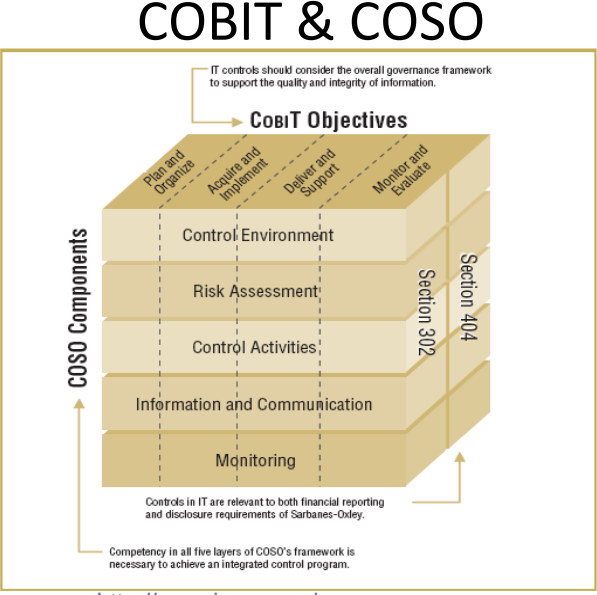
\includegraphics[scale=2.0]{res/img/cobit_coso_cube}
        \end{center}
        \caption{Grafico che mostra la relazione tra COBIT e COSO.}
        \label{fig:cobit:coso:relazione}
\end{figure}

\subsection{COBIT}
\label{COBIT}

\subsubsection{Pianificazione e organizzazione}

In un IT è importante definire un piano strategico per l'IT. Si è passati ad 
avere un insieme di applicazioni centralizzate ad una architetture distribuite 
\textit{cloud}-centriche. Chi ha visto queste innovazioni ieri oggi sta 
guadagnando un sacco.

L'\textit{information architecture} si focalizza su come viene distribuita 
l'informazione, su come viene distribuito il dato e su come aggiunge 
informazione al dato.

L'innovazione tecnologica è quella di andare verso un IT decentralizzato. La 
manutenzione è importante, ed è quindi importante capire che una rivisitazione 
dei costi IT non è possibile farla a costo 0. I processi messi in piedi sono 
molti importanti. La comunicazione è fondamentale, ed è un difetto di 
informatici e ingegneri. La non-comunicazione fanno appassire le 
idee\footnote{Perla del professore: \textbf{una buona idea comunicata bene 
ottiene molto di più di una idea eccellente comunicata male}}, e questo viene 
aggravato dall'inerzia che una grande azienda ha, in quanto un gran numero di 
persone si muovono lentamente tra loro.

Le risorse IT sono importanti anche loro: non serve più solo prendere ``quello 
bravo'', ma è importante avere un piano di \textit{retention}, ovvero capire 
come mantenere i dipendenti (soprattutto le persone chiave) all'interno 
dell'azienda. Questo andrebbe fatto anche nelle aziende piccole (20-30 
dipendenti)\footnote{Il professore consiglia di andare a vedere il PMI: 
\textit{Project Management Institute}, che spiega come gestire vari progetti.}.

\subsubsection{Acquisizione e implementazione}

È importante identificare soluzione automatizzate 


\subsubsection{Consegna e supporto}

Quando si hanno servizi di diverse parti gli SLI(?) sono fondamentali.
Gestione e capacità sono concetti diversi. Quando si ha settato 
un'organizzazione il limite estremo è la capacità ottimale (è quando tutti 
lavorano al 100\%, che è impossibile). Da qui bisogna capire dove si è e quanto 
ce n'è, e questo viene detto \textit{capacity}. Siccome è molto difficile per 
aziende grosse si guardano gli indicatori finanziari.
